\chapter{Results}\label{chap:results}

\subsection{Data Collection}

All results are saved in allcommits.json() \ref{fig:all-commits} file that we are required to create prior to executing the script. 
If the file is not created accordingly, the following error message is printed in the terminal: "The file is empty or does not exist."
\begin{figure}
    \centering
    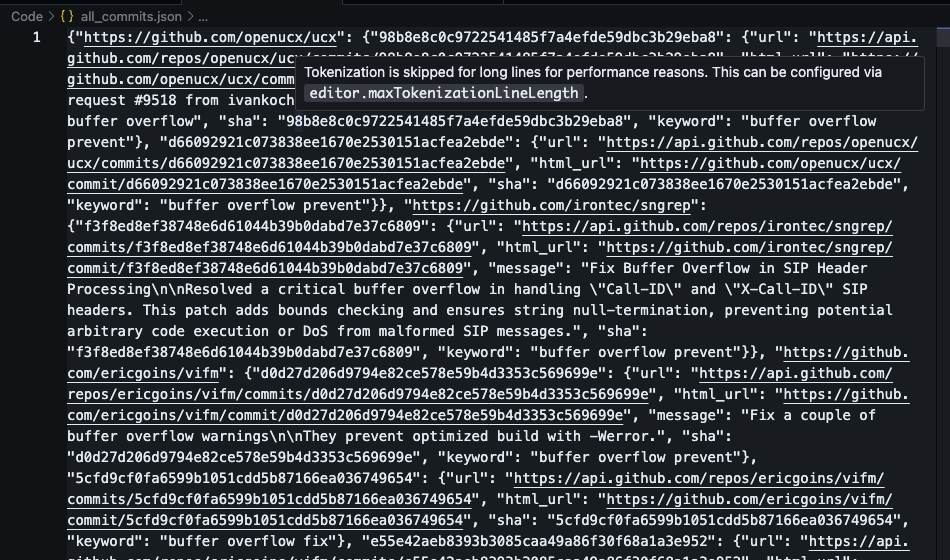
\includegraphics[width=1\linewidth]{all_commits.png}
    \caption{Scrapped Repositories}
    \label{fig:all-commits}
\end{figure}


\subsection{Keyword Filtering}

The result of \textbf{filterShowcase.py} is saved to the \textbf{DataFilter.json} file. It contains two JSON arrays for handling showcases and not showcases. The result is shown in figures \ref{fig:showcases_filtered} and \ref{fig:showcases_filtered}.

\begin{figure}
    \centering
    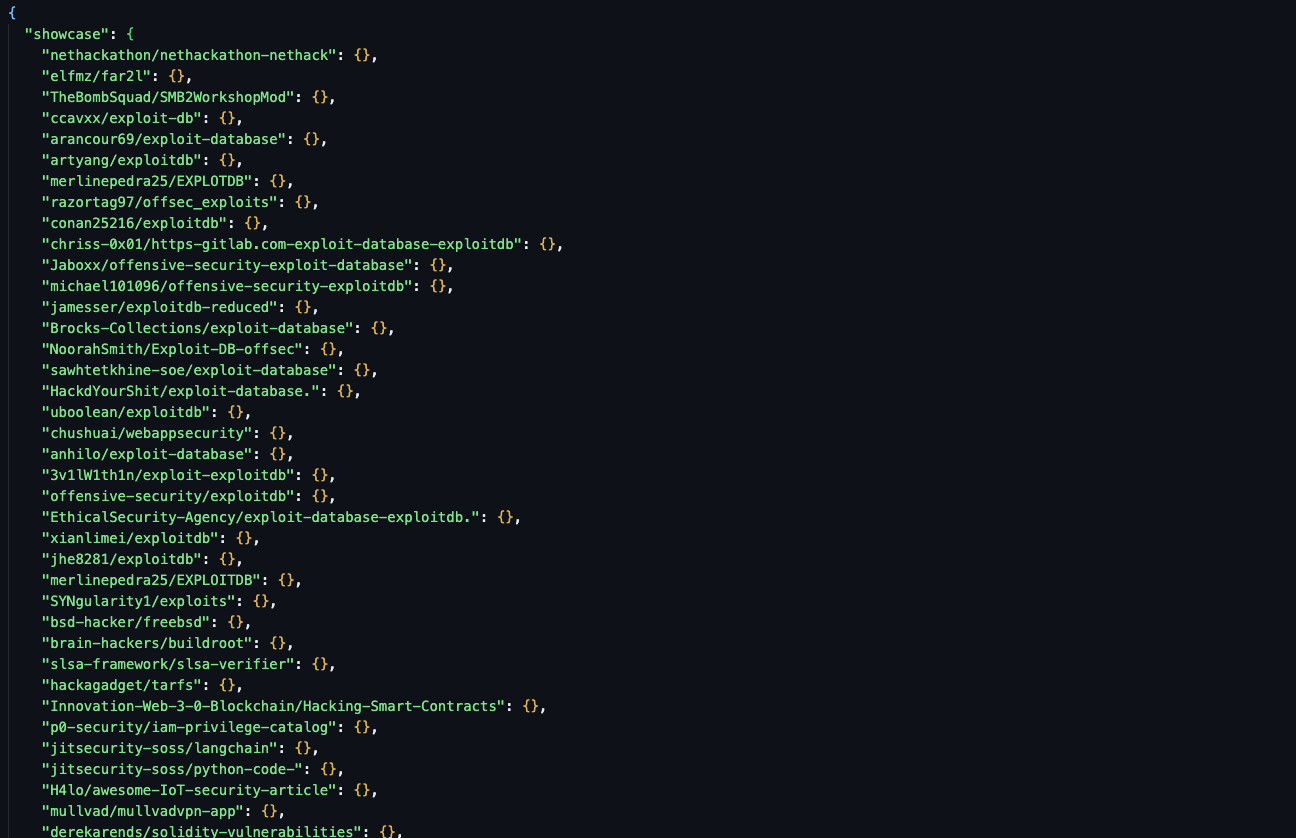
\includegraphics[width=1\linewidth]{showchase.png}
    \caption{Showcases filtered repositories}
    \label{fig:showcases_filtered}
\end{figure}

\begin{figure}
    \centering
    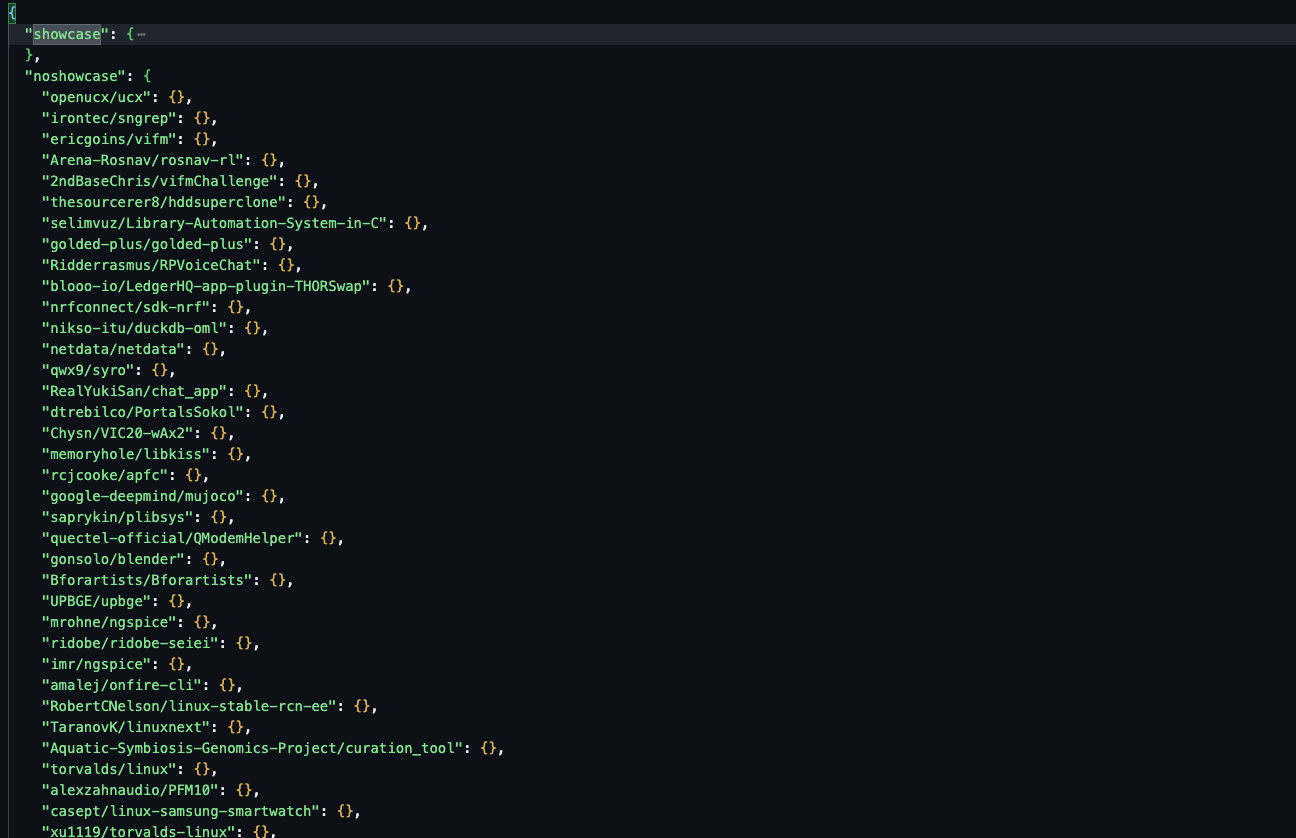
\includegraphics[width=1\linewidth]{noshowcase.png}
    \caption{No showcases filtered repositories}
    \label{fig:noshowcases_filtered}
\end{figure}

\subsection{Language Segregation}

The result, which separates those repositories with Python code from those without Python code, is also saved in the \textbf{DataFilter.json} file. 
The results have been saved in two separated JSON arrays with names \textbf{no-python} and \textbf{python}, as shown in Figures \ref{fig:python} and \ref{fig:no-python}.

\begin{figure}
    \centering
    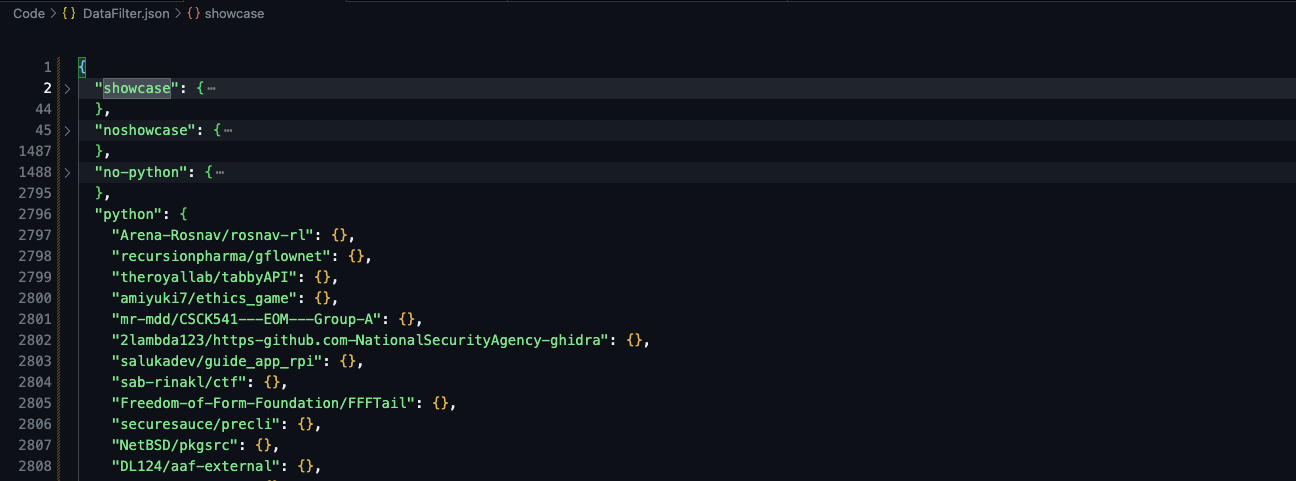
\includegraphics[width=1\linewidth]{python.png}
    \caption{Repositories with Python code}
    \label{fig:python}
\end{figure}

\begin{figure}
    \centering
    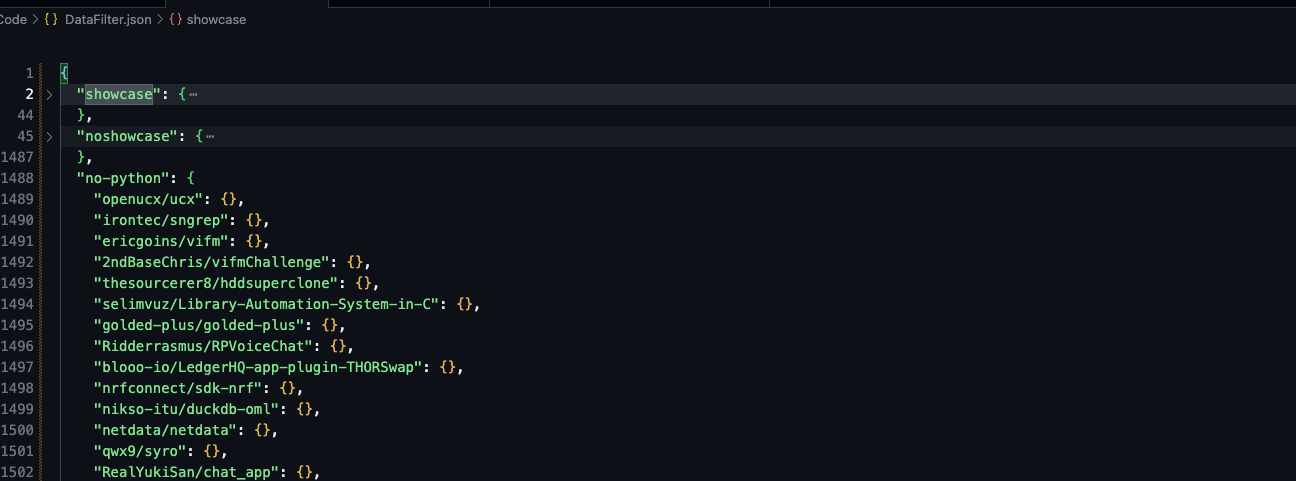
\includegraphics[width=1\linewidth]{no-python.png}
    \caption{Repositories without Python code}
    \label{fig:no-python}
\end{figure}

\subsection{Commit Analysis}

As mentioned before, the result of this step has been saved in the \textbf{PyCommitsWithDiffs.json} JSON file. 
The files are structured as JSON objects; each object is a repository, and commit diffs are located inside that. Figure \ref{fig:py-diffcommits} shows a sample of this step result.

\begin{figure}
    \centering
    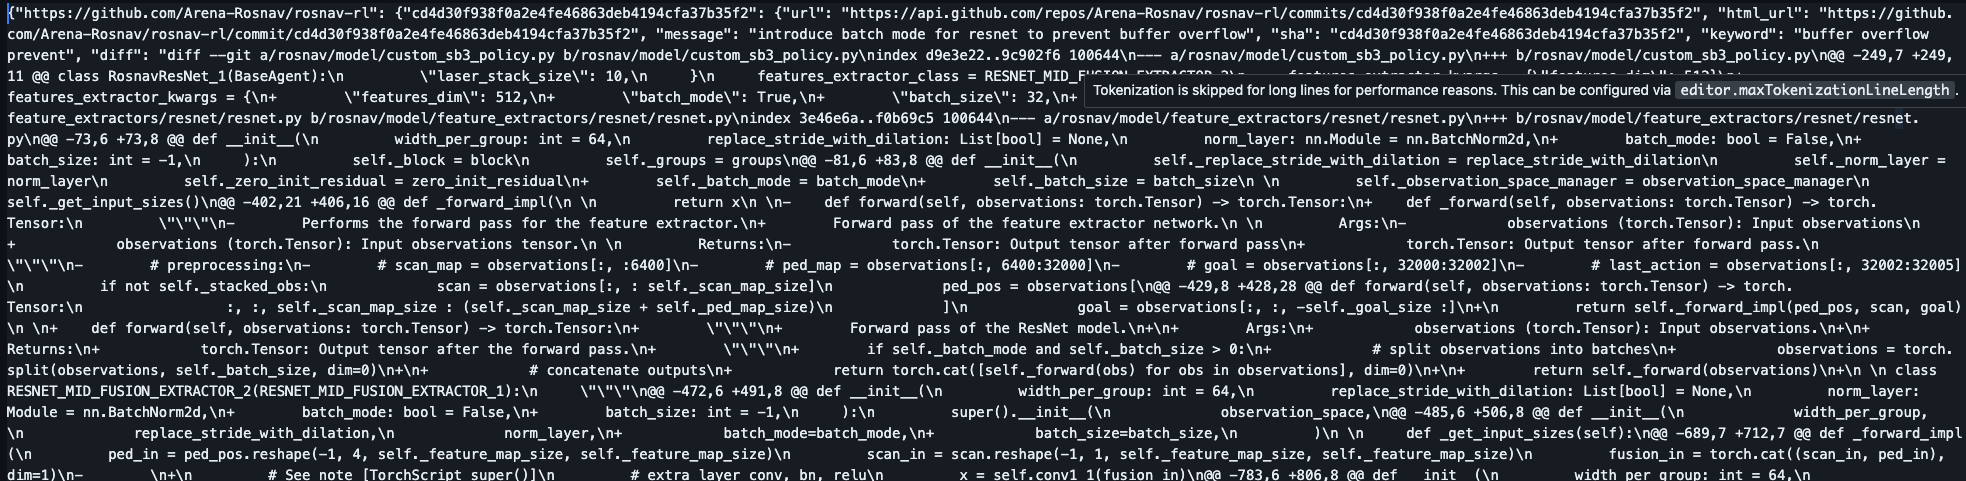
\includegraphics[width=1\linewidth]{PyDiffcommits.png}
    \caption{PyCommitsWithDiffs data}
    \label{fig:py-diffcommits}
\end{figure}

\subsection{Model Training}

Present the results of training the model on the augmented dataset, including model performance metrics, such as accuracy, precision, recall, F1-score, and any insights derived from the trained model's predictions.

